% Copyright (c) 2015 Daniele Masini - d.masini.it@gmail.com

\section{Esercizi}

\subsection{Esercizi riepilogativi}

\begin{esercizio}
\label{ese:2.1}
In base alla figura a lato rispondi alle seguenti domande\\
\begin{minipage}{.7\linewidth}
\begin{enumeratea}
\item Il lato $AB$ si oppone all'angolo \ldots\ldots\ldots
\item L'angolo $\alpha$ si oppone al lato \ldots\ldots\ldots
\item L'angolo di vertice $C$ si chiama \ldots\ldots\ldots
\item L'angolo $\gamma$ è adiacente ai lati \ldots\ldots{} e 
\ldots\ldots
\item I lati $AB$ e $BC$ sono adiacenti all'angolo \ldots\ldots
\item I lati $AC$ e $AB$ formano l'angolo \ldots\ldots
\item Traccia l'angolo esterno al triangolo nel vertice $A$
\item Traccia la bisettrice dell'angolo $\beta$
\item Traccia l'altezza relativa alla base $AB$
\item Traccia la mediana relativa al lato $BC$
\end{enumeratea}
\end{minipage}\hfil
\begin{minipage}{.3\linewidth}
%\begin{wrapfigure}{r}{0pt}
  \centering
    % Copyright (c) 2015 Daniele Masini - d.masini.it@gmail.com

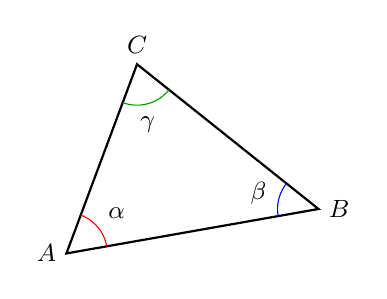
\begin{tikzpicture}[scale=1.3,font=\small]
\usetikzlibrary{calc}

\begin{scope}[rotate=10]
\coordinate (a) at (0,0);
\coordinate (c) at (1,1.7);
\coordinate (b) at (2.5,0);

\draw[thick] (b) node[right] {$B$} -- (c) node[above] {$C$} -- (a) node[left] {$A$} -- cycle;

\begin{scope}
\clip (a) -- (b) -- (c) -- cycle;
\draw[red] (a) circle (0.4);
\node at ([shift={(.55,.3)}]a) {$\alpha$};
\draw[blue] (b) circle (0.4);
\node at ([shift={(-.55,.25)}]b) {$\beta$};
\draw[green!60!black] (c) circle (0.4);
\node at ([shift={(0,-.6)}]c) {$\gamma$};
\end{scope}

\end{scope}

\end{tikzpicture}

%\end{wrapfigure}
\end{minipage}
\end{esercizio}

\begin{esercizio}
\label{ese:2.2}
Disegna un segmento $AB$, quindi disegna i triangoli $ABC$ e $ABD$ 
che hanno la base $AB$ in comune.
\end{esercizio}

\begin{esercizio}
\label{ese:2.3}
Disegna le tre altezze di ciascuno dei triangoli nella 
figura~\ref{fig:ese2.3}.
\end{esercizio}


\begin{inaccessibleblock}[Figura: TODO]
 \begin{figure}[htb]
\centering% Copyright (c) 2015 Daniele Masini - d.masini.it@gmail.com

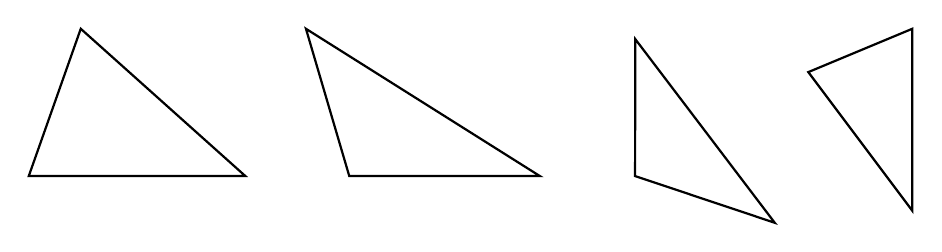
\begin{tikzpicture}[scale=1.1,font=\small]
\usetikzlibrary{calc}

\begin{scope}
\coordinate (a) at (0,0);
\coordinate (c) at (0.6,1.7);
\coordinate (b) at (2.5,0);
\draw[thick] (b)-- (c) -- (a) -- cycle;
\end{scope}

\begin{scope}[xshift=3.7cm]
\coordinate (a) at (0,0);
\coordinate (c) at (-.5,1.7);
\coordinate (b) at (2.2,0);
\draw[thick] (b)-- (c) -- (a) -- cycle;
\end{scope}

\begin{scope}[xshift=7cm, rotate=-18.5]
\coordinate (a) at (0,0);
\coordinate (c) at (-.5,1.5);
\coordinate (b) at (1.7,0);
\draw[thick] (b)-- (c) -- (a) -- cycle;
\end{scope}

\begin{scope}[xshift=9cm]
\coordinate (a) at (0,1.2);
\coordinate (c) at (1.2,1.7);
\coordinate (b) at (1.2,-0.4);
\draw[thick] (b)-- (c) -- (a) -- cycle;
\end{scope}


\end{tikzpicture}

\caption{Esercizio~\ref{ese:2.3}}\label{fig:ese2.3}
\end{figure}
\end{inaccessibleblock}

\begin{esercizio}
\label{ese:2.4}
Per ciascuna delle coppie di triangoli a lato indica se sono 
congruenti ed eventualmente per quale criterio.\\
\begin{minipage}{.5\linewidth}
\begin{enumeratea}
\item Si sa che sono congruenti i lati $AB$ con $A'B'$ e $AC$ con 
$A'C'$, l'angolo $\widehat{A}$ con l'angolo $\widehat{A'}$.\\
I triangoli sono congruenti?\tab	Sì\quad	No\\
Se sì, per il \ldots\ldots\ldots\ldots\ldots\ldots\ldots\ldots

\item Si sa che sono congruenti i lati $AB$ con $A'B'$ e gli angoli 
$\widehat{A}$ con $\widehat{B'}$ e $\widehat{B}$ con $\widehat{A'}$.\\
I triangoli sono congruenti?\tab	Sì\quad	No\\
Se sì, per il \ldots\ldots\ldots\ldots\ldots\ldots\ldots\ldots

\item Si sa che sono congruenti i lati $AB$ con $A'B'$ e $BC$ con 
$A'C'$, l'angolo $\widehat{A}$ con $\widehat{A'}$.\\
I triangoli sono congruenti?\tab	Sì\quad	No\\
Se sì, per il \ldots\ldots\ldots\ldots\ldots\ldots\ldots\ldots
\end{enumeratea}
\end{minipage}\hfil
\begin{minipage}{.4\linewidth}
  \centering
    % Copyright (c) 2015 Daniele Masini - d.masini.it@gmail.com

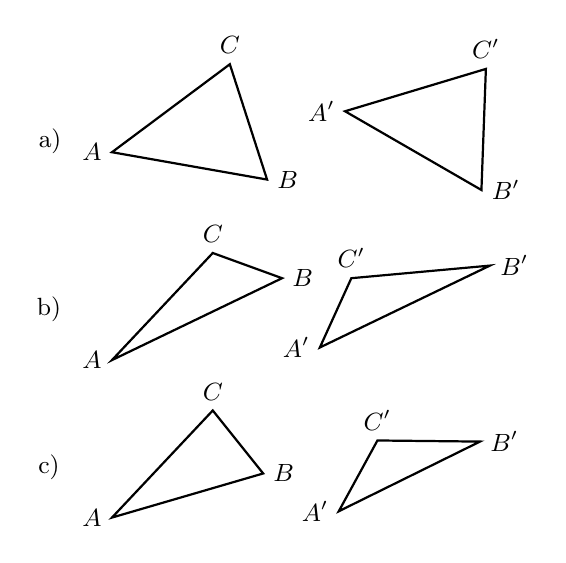
\begin{tikzpicture}[scale=0.8,font=\small]
\usetikzlibrary{calc}

\begin{scope}[rotate=-10]
\coordinate (a) at (0,0);
\coordinate (c) at (1.6,1.7);
\coordinate (b) at (2.5,0);
\draw[thick] (b) node[right] {$B$} -- (c) node[above] {$C$} -- (a) node[left] {$A$} -- cycle;
\node at (-1,0) {a)};
\end{scope}

\begin{scope}[xshift=3.7cm,yshift=0.65cm,rotate=-30]
\coordinate (a) at (0,0);
\coordinate (c) at (1.6,1.7);
\coordinate (b) at (2.5,0);
\draw[thick] (b) node[right] {$B'$} -- (c) node[above] {$C'$} -- (a) node[left] {$A'$} -- cycle;
\end{scope}

\begin{scope}[yshift=-3.3cm]
\coordinate (a) at (0,0);
\coordinate (c) at (1.6,1.7);
\coordinate (b) at (2.7,1.3);
\draw[thick] (b) node[right] {$B$} -- (c) node[above] {$C$} -- (a) node[left] {$A$} -- cycle;
\node at (-1,0.8) {b)};
\end{scope}

\begin{scope}[xshift=3.3cm,yshift=-3.1cm]
\coordinate (a) at (0,0);
\coordinate (c) at (0.5,1.1);
\coordinate (b) at (2.7,1.3);
\draw[thick] (b) node[right] {$B'$} -- (c) node[above] {$C'$} -- (a) node[left] {$A'$} -- cycle;
\end{scope}

\begin{scope}[yshift=-5.8cm]
\coordinate (a) at (0,0);
\coordinate (c) at (1.6,1.7);
\coordinate (b) at (2.4,0.7);
\draw[thick] (b) node[right] {$B$} -- (c) node[above] {$C$} -- (a) node[left] {$A$} -- cycle;
\node at (-1,0.8) {c)};
\end{scope}

\begin{scope}[xshift=3.6cm,yshift=-5.7cm,rotate=10]
\coordinate (a) at (0,0);
\coordinate (c) at (0.8,1);
\coordinate (b) at (2.4,0.7);
\draw[thick] (b) node[right] {$B'$} -- (c) node[above] {$C'$} -- (a) node[left] {$A'$} -- cycle;
\end{scope}


\end{tikzpicture}

\end{minipage}
\end{esercizio}

\begin{multicols}{2}

\subsubsection*{Dimostra le seguenti affermazioni, utilizzando il 
1\textsuperscript{o} e il 2\textsuperscript{o} criterio di congruenza 
dei triangoli.}

\begin{esercizio}
\label{ese:2.5}
In un triangolo $ABC$ prolunga la mediana $AM$ di un segmento $MD$ 
congruente a $MA$. Dimostra che il triangolo $AMC$ è congruente al 
triangolo $BMD$ e che il triangolo $ABM$ è congruente al triangolo 
$CMD$.
\end{esercizio}

\begin{esercizio}
\label{ese:2.6}
Due triangoli $ABC$ e $DEF$ hanno il lati $AB$ e $DE$ congruenti, 
hanno inoltre gli angoli esterni ai vertici $A$ e $B$ rispettivamente 
congruenti agli angoli esterni ai vertici $D$ ed $E$. Dimostra che i 
due triangoli sono congruenti.
\end{esercizio}

\begin{esercizio}
\label{ese:2.7}
Si consideri il segmento $AB$ e per il suo punto medio $M$ si tracci 
una retta $r$ qualsiasi. Su tale semiretta, da parti opposte rispetto 
ad $AB$, si prendano due punti $S$ e $T$ tali che $SM\cong MT$. 
Dimostrare che i triangoli $AMS$ e $TMB$ sono congruenti.
\end{esercizio}

\begin{esercizio}
\label{ese:2.8}
Due triangoli rettangoli sono congruenti se hanno rispettivamente 
congruenti i due cateti.
\end{esercizio}

\begin{esercizio}
\label{ese:2.9}
Due triangoli rettangoli sono congruenti se hanno congruenti un 
cateto e l'angolo acuto adiacente ad esso.
\end{esercizio}

\begin{esercizio}
\label{ese:2.10}
Due triangoli isosceli sono congruenti se hanno congruenti tra loro 
l'angolo al vertice e i due lati obliqui.
\end{esercizio}

\begin{esercizio}
\label{ese:2.11}
Nel triangolo isoscele $ABC$, di base $BC$, prolunga la bisettrice 
$AD$ di un segmento $DE$. Dimostra che $AE$ è bisettrice dell'angolo 
$B\widehat{E}C$.
\end{esercizio}

\begin{esercizio}
\label{ese:2.12}
Dati due triangoli congruenti $ABC$ e $A'B'C'$, si considerino sui 
lati $AC$ e $A'C'$ due punti $D$ e $D'$ tali che $DC\cong D'C'$.  
Dimostrare che $DB\cong D'B'$.
\end{esercizio}

\begin{esercizio}
\label{ese:2.13}
Siano $ABC$ e $DEF$ due triangoli congruenti. Sui lati congruenti 
$AB$ e $DE$ prendi il punto $G$ su $AB$ e $H$ su $DE$, in modo che 
$AG\cong DH$. Dimostra che anche $GC$ è congruente ad $HF$.
\end{esercizio}

\begin{esercizio}
\label{ese:2.14}
Del triangolo $ABC$ prolunga il lato $AB$ di un segmento $BD$ 
congruente a $BC$, analogamente prolunga il lato $CB$ di un segmento 
$BE$ congruente ad $AB$. Traccia la bisettrice dell'angolo 
$A\widehat{B}C$ e sia $F$ la sua intersezione con $AC$. Traccia la 
bisettrice dell'angolo $D\widehat{B}E$ e chiama $G$ la sua 
intersezione con $DE$. Dimostra che $BF\cong BG$.
\end{esercizio}

\begin{esercizio}
\label{ese:2.15}
Nel triangolo $ABC$ traccia la bisettrice $AD$ dell'angolo in $A$. 
Con origine in $D$ traccia due semirette che incontrano 
rispettivamente $AC$ in $E$ e $AB$ in $F$, in modo che 
$A\widehat{D}F\cong A\widehat{D}E$. Dimostra che il triangolo $AFE$ è 
un triangolo isoscele.
\end{esercizio}

\begin{esercizio}
\label{ese:2.16}
Nel triangolo $ABC$ con $AC<AB$ traccia la bisettrice $AD$ 
dell'angolo in $A$. Per il punto $D$ traccia la perpendicolare alla 
bisettrice $AD$. Detti $E$ ed $F$ i punti in cui la perpendicolare 
incontra rispettivamente i lati $AC$ e $AB$, dimostra che $AF\cong 
AE$.
\end{esercizio}

\begin{esercizio}
\label{ese:2.17}
Sui prolungamenti oltre $A$ del lato $AC$, oltre $B$ del lato $AB$ e 
oltre $C$ del lato $BC$ di un triangolo equilatero $ABC$ si 
considerino i segmenti congruenti $AA'$, $BB'$, $CC'$. Dimostrare che 
il triangolo $A'B'C'$ è ancora equilatero.
\end{esercizio}

\begin{esercizio}
\label{ese:2.18}
Dato l'angolo convesso $b\widehat{A}c$ si considerino su $b$ i due 
punti $B$ e $B'$ e su $c$ i punti $C$ e $C'$, tali che $AB$ e $AB'$ 
siano rispettivamente congruenti con $AC$ e $AC'$. Dimostrare che 
$BB'$ e $BC'$ sono rispettivamente congruenti con $CC'$ e $B'C$.
\end{esercizio}

\begin{esercizio}
\label{ese:2.19}
Dato un segmento $AB$, condurre per il suo punto medio $M$ una 
qualsiasi retta $r$ e considerare su di essa, da parti opposte 
rispetto ad $AB$, due segmenti congruenti $MC$ e $MD$. Dimostrare che 
i triangoli $AMC$ e $BMD$ sono congruenti.
\end{esercizio}

\begin{esercizio}
\label{ese:2.20}
Sui lati dell'angolo $X\widehat{O}Y$ si considerino i punto $A$ e $B$ 
tali che $OA\cong OB$. Sia $H$ un punto della bisettrice dell'angolo 
tale che $OH<OA$. Siano $T$ il punto di intersezione di $AH$ con $OY$ 
e $S$ il punto di intersezione di $BH$ con $OX$. Dimostrare che 
$AH\cong HB$ e $SH\cong HT$.
\end{esercizio}

\begin{esercizio}
\label{ese:2.21}
Si consideri un punto $O$ interno al triangolo $ABC$ e si congiunga 
tale punto con i vertici $A$ e $B$ del triangolo. Si prolunghino i 
segmenti $AO$ e $BO$ oltre $O$ di due segmenti $OA'$ e $OB'$ 
rispettivamente congruenti ai suddetti segmenti. Dimostrare che i 
segmenti $AB$ e $A'B'$ sono congruenti.
\end{esercizio}

\begin{esercizio}
\label{ese:2.22}
Si considerino i triangoli congruenti $ABC$ e $A'B'C'$ e si 
prolunghino i lati $AB$ e $A'B'$ di due segmenti $BP$ e $B'P'$ tra 
loro congruenti. Si prolunghino inoltre i lati $AC$ e $A'C'$ di due 
segmenti $CQ$ e $C'Q'$ tra loro congruenti. Si dimostri che sono 
congruenti i triangoli $CPQ$ e $C'P'Q'$.
\end{esercizio}

\begin{esercizio}
\label{ese:2.23}
Sui lati $a$ e $b$ di un angolo di vertice $O$ prendi i punti $A$ e 
$B$ sulla semiretta $a$ e i punti $C$ e $D$ sulla semiretta $b$, in 
modo che $OA\cong OC$ e $AB\cong CD$. Sia $E$ il punto di 
intersezione di $AD$ con $BC$. Dimostra che sono congruenti i 
triangoli $ABE$ e $CDE$.
\end{esercizio}

\begin{esercizio}
\label{ese:2.24}
Sia $C$ un punto della bisettrice dell'angolo convesso 
$a\widehat{O}b$, $A$ un punto sul lato $a$ e $B$ un punto sul lato 
$b$, tali che $OA\cong OB$. Dimostra che i triangoli $BCO$ e $ACO$ 
sono congruenti.
\end{esercizio}

\begin{esercizio}
\label{ese:2.25}
Dato un triangolo $ABC$, traccia la parallela ad $AC$ passante per 
$B$ e la parallela a $BC$ passante per $A$. Indica con $D$ il punto 
di intersezione delle due rette tracciate. Dimostra che i triangoli 
$ABC$ e $ABD$ sono congruenti.
\end{esercizio}

\begin{esercizio}
\label{ese:2.26}
Dato il triangolo $ABC$, costruire esternamente a esso i triangoli 
equilateri $ACD$ e $BCE$. Dimostra che $AE=BD$.
\end{esercizio}

\begin{esercizio}
\label{ese:2.27}
In un triangolo $ABC$, sul prolungamento del lato $AB$, dalla parte 
di $B$, prendi un punto $D$ tale che $BD\cong AB$, analogamente sul 
prolungamento del lato $CB$, dalla parte di $B$, prendi un punto $E$ 
tale che $EB\cong BC$. Dimostra che la mediana $BM$ del triangolo 
$ABC$ è allineata con la mediana $BN$ del triangolo $DBE$, ossia che 
l'angolo formato dalle due mediane è un angolo piatto.
\end{esercizio}

\subsubsection*{Dimostra le seguenti affermazioni sui triangoli 
isosceli.}

\begin{esercizio}
\label{ese:2.28}
In un triangolo isoscele le mediane relative ai lati congruenti sono 
congruenti. 
\end{esercizio}

\begin{esercizio}
\label{ese:2.29}
In un triangolo isoscele le bisettrici degli angoli alla base sono 
congruenti. 
\end{esercizio}

\begin{esercizio}
\label{ese:2.30}
Due triangoli isosceli sono congruenti se hanno rispettivamente 
congruenti l'angolo al vertice e uno dei lati obliqui.
\end{esercizio}

\begin{esercizio}
\label{ese:2.31}
Due triangoli isosceli sono congruenti se hanno rispettivamente 
congruenti la base e uno degli angoli ad essa adiacenti.
\end{esercizio}

\begin{esercizio}
\label{ese:2.32}
Due triangoli isosceli sono congruenti se hanno rispettivamente 
congruenti la base e la bisettrice dell'angolo al vertice.
\end{esercizio}

\begin{esercizio}
\label{ese:2.33}
Due triangoli isosceli sono congruenti se hanno rispettivamente 
congruenti gli angoli al vertice e due lati corrispondenti qualsiasi.
\end{esercizio}

\begin{esercizio}
\label{ese:2.34}
Sia $P$ il punto di intersezione delle bisettrici degli angoli alla 
base $AB$ di un triangolo isoscele $ABC$. Dimostra che anche $APB$ è 
isoscele.
\end{esercizio}

\begin{esercizio}
\label{ese:2.35}
In un triangolo isoscele $ABC$ di base $AB$ e vertice $C$, prendi su 
$AC$ un punto $M$ e su $BC$ un punto $N$ in modo che $CM\cong CN$. 
Quali delle seguenti coppie di triangoli sono congruenti? Dimostralo.
\begin{multicols}{2}
\begin{enumeratea}
\item $ACN$ e $ANB$
\item $ACN$ e $BCM$
\item $ABN$ e $ABM$
\item $ABC$ e $MNC$
\end{enumeratea}
\end{multicols}
\end{esercizio}

\begin{esercizio}
\label{ese:2.36}
In un triangolo isoscele $ABC$ di base $AB$ e vertice $C$, indica con 
$M$ il punto medio di $AC$, con $N$ il punto medio di $CB$ e con $H$ 
il punto medio di $AB$. Quali delle seguenti coppie di triangoli sono 
congruenti? Dimostralo.
\begin{multicols}{2}
\begin{enumeratea}
\item $AMH$ e $HNB$
\item $MNH$ e $MNC$
\item $AMH$ e $MCN$
\end{enumeratea}
\end{multicols}
\end{esercizio}

\begin{esercizio}
\label{ese:2.37}
Sui lati $AC$ e $CB$ del triangolo isoscele $ABC$ di base $AB$ 
considera rispettivamente due punti $D$ ed $E$ tali che $CD\cong CE$. 
Dimostra che i triangoli $ADB$ e $AEB$ sono congruenti. Detto $P$ il 
punto di intersezione tra $AE$ e $DB$, dimostrare che $ABP$ e $DPE$ 
sono triangoli isosceli.
\end{esercizio}

\begin{esercizio}
\label{ese:2.38}
In un triangolo isoscele $ABC$ di base $AB$ e vertice $C$ prolunga la 
base $AB$, dalla parte di $A$ di un segmento $AD$ e dalla parte di 
$B$ di un segmento $BE$ congruente ad $AD$. Dimostra che anche il 
triangolo $DEC$ è isoscele.
\end{esercizio}

\begin{esercizio}
\label{ese:2.39}
Nel triangolo isoscele $ABC$ di base $BC$, prendi sul prolungamento 
di $BC$ due segmenti congruenti $BQ$ e $CP$. Dimostra che $APB$ è 
isoscele.
\end{esercizio}

\begin{esercizio}
\label{ese:2.40}
Due triangoli isosceli $ABC$ e $ABD$ hanno in comune la base $AB$, i 
vertici $C$ e $D$ sono situati da parti opposte rispetto alla base 
$AB$. Dimostra che la retta per $CD$ è bisettrice dell'angolo in $C$.
\end{esercizio}

\begin{esercizio}
\label{ese:2.41}
In un triangolo isoscele $ABC$ di base $AB$ e vertice $C$ traccia le 
bisettrici $BD$ all'angolo in $B$ e $AE$ all'angolo in $A$. Dimostra 
che $BD\cong AE$. Detto $O$ il punto di intersezione delle bisettrici 
dimostra che $AOB$ è isoscele. Dimostra che il triangolo $ADO$ è 
congruente al triangolo $BEO$.
\end{esercizio}

\begin{esercizio}
\label{ese:2.42}
In un triangolo isoscele $ABC$ di base $AB$ e vertice $C$ prolunga, 
dalla parte di $C$ la bisettrice $CD$ dell'angolo in $C$ di un 
segmento $CE$. Dimostra che $ED$ è bisettrice dell'angolo 
$A\widehat{E}D$.
\end{esercizio}

\begin{esercizio}
\label{ese:2.43}
In un triangolo isoscele $ABC$ di base $AB$ e vertice $C$ prendi su 
$AC$ un punto $D$ e su $BC$ il punto $E$ tali che $AD\cong BE$. Detto 
$O$ il punto di intersezione di $AE$ con $BD$, dimostra che $AOB$ è 
isoscele.
\end{esercizio}

\begin{esercizio}
\label{ese:2.44}
In un triangolo $ABC$ sia $M$ il punto medio di $AB$. Traccia la 
mediana $CM$ e prolungala dalla parte di $M$ di un segmento $MD$ 
congruente a $CM$. Dopo aver dimostrato che il triangolo $AMC$ è 
congruente a $BMD$, dimostra che se $CM$ è bisettrice dell'angolo in 
$C$ allora $ABC$ è isoscele.
\end{esercizio}

\begin{esercizio}
\label{ese:2.45}
In un triangolo isoscele $ABC$ di base $AB$ e vertice $C$, prendi su 
$AC$ un punto $D$ e su $CB$ un punto $E$ in modo che $CD\cong CE$. 
Dimostra che il triangolo $DME$, dove $M$ è il punto medio della base 
$AB$, è isoscele.
\end{esercizio}

\begin{esercizio}
\label{ese:2.46}
Due triangoli isoscele hanno in comune la base, dimostra che la retta 
che unisce i vertici dei due triangoli divide la base a metà.
\end{esercizio}

\begin{esercizio}
\label{ese:2.47}
In un triangolo isoscele $ABC$ di base $AB$ e vertice $C$, si ha che 
$AC\cong CB\cong 2\cdot AB$. Indica con $M$ il punto medio di $AC$ e 
$N$ il punto medio di $BC$, $P$ il punto di intersezione di $BM$ con 
$AN$. Individua tutti i triangoli isosceli che si vengono a formare. 
Dimostra che $ACN$ è congruente a $BCM$, che $ABP$ è isoscele, che 
$P$ appartiene all'altezza $CH$ del triangolo.
\end{esercizio}

\begin{esercizio}
\label{ese:2.48}
Sia dato il triangolo $ABC$ e sia $M$ il punto medio del lato $AB$. 
Si prolunghi $CM$ di un segmento $MD\cong CM$. Dimostrare che 
$A\widehat{C}B\cong A\widehat{D}B$.
\end{esercizio}

\begin{esercizio}
\label{ese:2.49}
Si prolunghino i lati $AC$ e $CB$ del triangolo isoscele $ABC$ 
rispettivamente di due segmenti $CP$ e $CQ$ tra loro congruenti. 
Dimostrare che $A\widehat{Q}B\cong A\widehat{P}Q$ e che 
$A\widehat{B}P\cong Q\widehat{A}B$.
\end{esercizio}

\begin{esercizio}
\label{ese:2.50}
Sulla base $AB$ di un triangolo isoscele $ABC$ prendi i punti $M$ e 
$N$ tali che $AM<AN$ e $AM\cong NB$. Dimostra che $CMN$ è isoscele.
\end{esercizio}

\begin{esercizio}
\label{ese:2.51}
Sia $D$ il punto di intersezione delle bisettrici degli angoli alla 
base di un triangolo isoscele $ABC$ di vertice $A$. Dimostra che 
$BDC$ è isoscele.
\end{esercizio}

\begin{esercizio}
\label{ese:2.52}
Nel triangolo isoscele $ABC$ di base $BC$ prolunga $AB$ di un 
segmento $BD$ e $AC$ di un segmento $CE$ in modo che $DE\cong CE$. 
Dimostra che $BE\cong DC$.
\end{esercizio}

\begin{esercizio}
\label{ese:2.53}
Sia $ABC$ un triangolo isoscele con $AB\cong AC$. Sui lati obliqui 
$AB$ e $AC$ costruisci, esternamente al triangolo, i triangoli 
equilateri $ABD$ e $ACE$. Congiungi $B$ con $E$ e $C$ con $D$. Detto 
$F$ il punto di intersezione di $DC$ e $BE$, dimostra che $BFC$ è 
isoscele.
\end{esercizio}

\subsubsection*{Esercizi sui criteri di congruenza dei triangoli e 
sui triangoli isosceli.}

\begin{esercizio}
\label{ese:2.54}
Due triangoli sono congruenti se hanno
\begin{enumeratea}
\item tre lati congruenti \hfill\boxV\quad\boxF
\item tre angoli congruenti \hfill\boxV\quad\boxF
\item due lati e l'angolo compreso congruenti\tab\hfill\boxV\quad\boxF
\item due angoli e il lato in comune 
congruenti\tab\hfill\boxV\quad\boxF
\item un lato e l'angolo opposto 
congruenti\tab\tab\hfill\boxV\quad\boxF
\end{enumeratea}
\end{esercizio}

\begin{esercizio}
\label{ese:2.55}
Prolunga nello stesso verso i lati di un triangolo equilatero di tre 
segmenti tra loro congruenti. Dimostra che il triangolo ottenuto 
congiungendo gli estremi dei segmenti aggiunti è equilatero.
\end{esercizio}

\begin{esercizio}
\label{ese:2.56}
Due triangoli equilateri sono congruenti se hanno lo stesso perimetro.
\end{esercizio}

\begin{esercizio}
\label{ese:2.57}
Dimostra che due triangoli equilateri che hanno in comune la base 
sono congruenti.
\end{esercizio}

\begin{esercizio}
\label{ese:2.58}
Se in due triangoli sono congruenti due coppie di lati e la mediana 
relativa ad uno di essi, allora i due triangoli sono congruenti.
\end{esercizio}

\begin{esercizio}
\label{ese:2.59}
Se in due triangoli sono congruenti due coppie di lati e la 
bisettrice relativa ad uno di essi, allora i due triangoli sono 
congruenti.
\end{esercizio}

\begin{esercizio}
\label{ese:2.60}
Due triangoli isosceli sono congruenti se hanno rispettivamente 
congruenti la base e un altro lato.
\end{esercizio}

\begin{esercizio}
\label{ese:2.61}
Se due triangoli hanno congruenti due lati e la mediana relativa a 
uno di essi allora sono congruenti.
\end{esercizio}

\begin{esercizio}
\label{ese:2.62}
In un triangolo se la bisettrice di un angolo è anche meddiana allora 
il triangolo è isoscele.
\end{esercizio}

\begin{esercizio}
\label{ese:2.63}
In un triangolo isoscele $ABC$ di base $BC$ e vertice $A$ prendi un 
punto $D$ sul lato $AB$ e un punto $E$ sul lato $AC$, in modo che 
$BD\cong EC$, unisci $C$ con $D$ e $B$ con $E$. Sia $F=BE\cap DC$. 
Dimostra che i triangoli $BFA$ e $CFA$ sono congruenti.
\end{esercizio}

\begin{esercizio}
\label{ese:2.64}
Dimostra che, prolungando i lati congruenti $AB$ e $AC$ di un 
triangolo isoscele di due segmenti congruenti rispettivamente $AP$ e 
$AQ$, si ha che $BQ\cong PC$.
\end{esercizio}

\begin{esercizio}
\label{ese:2.65}
In un triangolo isoscele $ABC$ di base $BC$ e vertice $A$, prolunga 
il lato $AB$ di un segmento $BD$ e il lato $AC$ di un segmento $CE$ 
in modo che $BD\cong CE$, prolunga la base $BC$ di un segmento $BG$, 
dalla parte di $B$, e di un segmento $CF$ dalla parte di $C$, in modo 
che $BG\cong CF$. Dimostra che sono congruenti i triangoli $ADG$ e 
$AEF$.
\end{esercizio}

\begin{esercizio}
\label{ese:2.66}
In un triangolo scaleno $ABC$ sia $AC>BC$. Prolunga $BC$, dalla parte 
di $C$, di un segmento $CD$ congruente ad $AC$ e prolunga $AC$, dalla 
parte di $C$, di un segmento $CE$ congruente a $BC$. Detto $H$ il 
punto di intersezione della retta per $AB$ con la retta per $DE$, 
dimostra che $AH\cong DH$.
\end{esercizio}

\begin{esercizio}
\label{ese:2.67}
In un triangolo isoscele $ABC$ di base $BC$ e vertice $A$, prolunga 
il lato $AB$ di un segmento $BD$ e il lato $AC$ di un segmento $CE$ 
in modo che $BD\cong CE$. Unisci $D$ con $C$ e prolunga il segmento 
$DC$, dalla parte di $C$ di un segmento $CF$. Unisci $E$ con $B$ e 
prolunga il segmento $EB$ dalla parte di $B$ di un segmento $BG\cong 
CF$. Dimostra che i triangoli $AGD$ e $AFE$ sono congruenti.
\end{esercizio}

\begin{esercizio}
\label{ese:2.68}
Dato il triangolo convesso non piatto $a\widehat{O}b$ si prenda un 
punto $A$ sul lato $Oa$ e un punto $B$ sul lato $Ob$, in modo che 
$OA\cong OB$. Sia $M$ il punto medio di $OA$ e $N$ il punto medio di 
$OB$, congiungi $A$ con $N$ e $B$ con $M$, indica con $P$ in punto di 
intersezione. Dimostra che sono congruenti i triangoli $OBC$ e $OAD$ 
e i triangoli $AOP$ e $OPB$.
\end{esercizio}

\begin{esercizio}
\label{ese:2.69}
Nel triangolo isoscele $ABC$ di base $AB$ e vertice $C$, prendi un 
punto $D$ sulla bisettrice $CH$ dell'angolo al vertice $C$, indica 
con $E$ il punto di intersezione della retta $AD$ con $BC$ e $F$ il 
punto di intersezione di $BD$ con $AC$. Dimostra che i triangoli $FDA$ 
e $EDB$ sono congruenti.
\end{esercizio}

\begin{esercizio}
\label{ese:2.70}
Siano $ABC$ e $ABD$ due triangoli isosceli aventi la base $AB$ in 
comune e i vertici $C$ e $D$ situati da parti opposte rispetto ad 
$AB$. Dimostrare che $A\widehat{C}D\cong D\widehat{C}B$.
\end{esercizio}

\begin{esercizio}
\label{ese:2.71}
Sia $P$ un punto interno al triangolo isoscele $ABC$ di base $AB$ e 
sia $AP\cong PB$. Si dimostri che $CP$ appartiene alla bisettrice 
dell'angolo in $C$.
\end{esercizio}

\begin{esercizio}
\label{ese:2.72}
Due triangoli equilateri $ABC$ e $DBC$ hanno la base $BC$ in comune e 
i vertici $A$ e $D$ situati da parti opposte rispetto alla base $BC$. 
Dimostra che i due triangoli sono congruenti.
\end{esercizio}

\begin{esercizio}
\label{ese:2.73}
Siano $ABC$ e $A'B'C'$ due triangoli congruenti. Si fissino su $AC$ 
un punto $P$ e su $A'C'$ un punto $P'$ tali che $AP\cong A'P'$. Si 
fissino su $BC$ un punto $Q$ e su $B'C'$ un punto $Q'$ tali che 
$BQ\cong B'Q'$. Si dimostri che $PQ\cong P'Q'$.
\end{esercizio}

\begin{esercizio}
\label{ese:2.74}
Nel triangolo generico $ABC$ sia $AK$ la bisettrice dell'angolo in 
$A$. Sul prolungamento dei lati $AB$ e $AC$, rispettivamente dalla 
parte di $B$ e dalla parte di $C$, individua due punti $D$ ed $E$, 
tali che $AD$ sia congruente ad $AE$. Dimostra che $DK$ è congruente 
a $KE$.
\end{esercizio}

\begin{esercizio}
\label{ese:2.75}
Due triangoli, che hanno un lato congruente e hanno congruenti anche 
i due angoli esterni al triangolo aventi per vertici gli estremi del 
lato congruente, sono congruenti. 
\end{esercizio}

\begin{esercizio}
\label{ese:2.76}
Dato il triangolo $ABC$ e un punto $O$ esterno al triangolo, si 
unisca $O$ con $A$, con $B$ e con $C$. Si prolunghi ciascun segmento, 
dalla parte di $O$, dei segmenti $OA'\cong OA$, $OB'\cong OB$, 
$OC'\cong OC$. Dimostra che $ABC\cong A'B'C'$.
\end{esercizio}

\begin{esercizio}
\label{ese:2.77}
Siano $LMN$ i punti medi dei lati del triangolo isoscele $ABC$, 
dimostra che anche $LMN$ è isoscele.
\end{esercizio}

\begin{esercizio}
\label{ese:2.78}
Siano $MN$ i punti medi dei lati congruenti $AB$ e $AC$ del triangolo 
isoscele $ABC$, dimostra che le mediane $AM$ e $AN$ sono congruenti.
\end{esercizio}

\begin{esercizio}
\label{ese:2.79}
Siano $A\widehat{O}B$ e $B\widehat{O}C$ due angoli consecutivi 
congruenti, sia $OM$ la bisettrice dell'angolo $A\widehat{O}B$. Sulle 
semirette $OC$, $OB$, $OM$ e $OA$ si prendano rispettivamente i 
segmenti tutti congruenti tra di loro $OC'$, $OB'$, $OM'$, $OA'$. 
Dimostrare che $A'M'\cong M'B'$ e $A'B'\cong B'C'$.
\end{esercizio}

\begin{esercizio}
\label{ese:2.80}
Sia $OM$ la bisettrice dell'angolo $A\widehat{O}B$. Sul lato 
dell'angolo $A\widehat{O}B$ si prendano i punti $P$ e $Q$ tali che 
$OP\cong OQ$. Sia $C$ un punto qualsiasi della bisettrice $OM$. 
Dimostra che $CP\cong CQ$.
\end{esercizio}

\begin{esercizio}
\label{ese:2.81}
Sia $P$ un punto interno al triangolo isoscele $ABC$, di base $AB$. 
Dimostra che se $P\widehat{A}C\cong P\widehat{C}B$ allora $P$ si 
trova sulla bisettrice dell'angolo in $A$.
\end{esercizio}

\begin{esercizio}
\label{ese:2.82}
Traccia la bisettrice a dell'angolo in $A$ del triangolo $ABC$ con 
$AB>AC$. Sulla bisettrice $a$ individua due punti $D$ ed $E$ tali che 
$AD\cong AB$ e $AE\cong AC$. Dimostra che i triangoli $ACD$ e $ABE$ 
sono congruenti.
\end{esercizio}

\begin{esercizio}
\label{ese:2.83}
In un triangolo $ABC$ con $AB>AC$ disegna la bisettrice $AD$ 
dell'angolo in $A$. Dal punto $D$ disegna una semiretta che taglia il 
triangolo $ABC$ e forma con $AD$ un angolo congruente a 
$A\widehat{D}C$. Questa semiretta incontra $AB$ in $E$. Dimostra che 
$CD$ e $DE$ sono congruenti.
\end{esercizio}

\begin{esercizio}
\label{ese:2.84}
Sia $ABC$ triangolo isoscele di base $BC$, prolunga i lati $AB$ dalla 
parte di $B$ e $AC$ dalla parte di $C$. Traccia la bisettrice $b$ 
dell'angolo esterno in $B$ e la bisettrice $c$ dell'angolo esterno in 
$C$. Queste bisettrici incontrano i prolungamenti dei lati, 
precisamente $c$ incontra il prolungamento di $AB$ in $E$ e $b$ 
incontra il prolungamento di $AC$ in $D$. Dimostra che $EC\cong BD$. 
Sia $F$ il punto di intersezione di $EC$ con $BD$, dimostra che $AF$ 
è la bisettrice dell'angolo in $A$.
\end{esercizio}

\begin{esercizio}
\label{ese:2.85}
Sia $ABC$ un triangolo isoscele di vertice $C$. Sul prolungamento di 
$AB$ si prenda $D$ dalla parte di $A$ ed $E$ dalla parte di $B$, in 
modo che $AD\cong BE$. Dimostra che $CDE$ è isoscele.
\end{esercizio}

\begin{esercizio}
\label{ese:2.86}
Sia $ABC$ un triangolo qualsiasi e sia $AL$ la bisettrice dell'angolo 
in $A$. Da $L$ si conduca la perpendicolare ad $AL$, essa incontra la 
retta $AB$ in $D$ e la retta $AC$ in $E$. Dimostra che $ADE$ è 
isoscele.
\end{esercizio}

\begin{esercizio}
\label{ese:2.87}
In un triangolo qualsiasi $ABC$, si prolunghi il lato $AB$ dalla 
parte di $B$ di un segmento $BD$ congruente ad $AB$ e si prolunghi il 
lato $BC$ dalla parte di $B$ di un segmento $BE$ congruente a $BC$. 
Detto $M$ il punto medio di $AC$ e $N$ il punto medio di $ED$, 
dimostra che $B$ appartiene alla retta per $MN$ (è sufficiente 
dimostrare che l'angolo $MBN$ è piatto).
\end{esercizio}

\begin{esercizio}
\label{ese:2.88}
Si prolunghino i lati congruenti $AC$ e $BC$ di un triangolo 
isoscele, rispettivamente di due segmenti congruenti $AD$ e $BE$. 
Detto $F$ il punto di intersezione di $AE$ con $DB$, dimostra che 
$FC$ è bisettrice dell'angolo in $C$.
\end{esercizio}

\begin{esercizio}
\label{ese:2.89}
Sulla bisettrice $c$ di un angolo $a\widehat{O}b$ prendi un punto $P$ 
e traccia da esso le perpendicolari ai lati $a$ e $b$ dell'angolo che 
incontrano rispettivamente in $A$ e in $B$ i suddetti lati. Dimostra 
che $OA\cong OB$.
\end{esercizio}

\begin{esercizio}
\label{ese:2.90}
In un triangolo isoscele di base $BC$ traccia due semirette aventi 
origine rispettivamente in $B$ e in $C$ e che incontrano $AB$ in $D$ 
e $AC$ in $E$. Dimostra che se le semirette si incontrano in un punto 
della mediana $AM$ relativa alla base $BC$ allora $AD\cong AE$.
\end{esercizio}

\begin{esercizio}
\label{ese:2.91}
$ABC$ è un triangolo isoscele con $AC$ congruente a $BC$; $M$ il 
punto medio di $AB$, $L$ il punto medio di $AC$ e $N$ il punto medio 
di $BC$. Sulla mediana $CM$ prendi un punto $K$ in modo che $KM<CK$. 
Sia $P$ il punto di intersezione di $NK$ con $AB$ e $Q$ il punto di 
intersezione di $LK$ con $AB$. Dimostra che $KPQ$ è un triangolo 
isoscele.
\end{esercizio}

\begin{esercizio}
\label{ese:2.92}
Dato il triangolo isoscele $ABC$ di base $BC$ e angolo in $A$ acuto 
traccia le altezze $BL$ e $CK$ relative ai lati obliqui. Prolunga 
$BL$ di un segmento $LD$ congruente a metà $BL$ e prolunga $CK$ di un 
segmento $EK$ congrunete a metà $KC$. Sia $F$ il punto di 
intersezione di $EB$ con $DC$. Dimsotra che $DEF$ è un triangolo 
isoscele.
\end{esercizio}

\begin{esercizio}
\label{ese:2.93}
Sugli assi dei lati di un triangolo equilatero si prendono tre punti 
interni al triangolo equidistanti dai vertici del triangolo. Dimostra 
che il triangolo che ha per vertici questi tre punti è anch'esso 
equilatero.
\end{esercizio}

\begin{esercizio}
\label{ese:2.94}
Sui lati $AB$, $BC$ e $CA$ di un triangolo equilatero si prendono tre 
punti $P$, $Q$, $R$ in modo che $AP$, $BQ$ e $CR$ siano congruenti 
tra di loro. Unisci i punti $P$, $Q$ e $R$ con i vertici opposti. 
Dimostra che questi segmenti si incontrano in tre punti che sono 
vertici di un triangolo equilatero.
\end{esercizio}

\begin{esercizio}
\label{ese:2.95}
Sia $ABCDE$ un pentagono regolare, ossia con tutti i lati congruenti 
e tutti gli angoli interni congruenti. Dal vertice $A$ traccia le due 
diagonali $AD$ e $AC$. Il pentagono resta così diviso in tre 
triangoli. Individua i due triangoli congruenti e dimostra che sono 
congruenti.
\end{esercizio}


\end{multicols}

\begin{esercizio}[Prove invalsi 2006]
\label{ese:2.99}
Osserva la figura a lato. Se $AB\not\cong AC$ e $BH\cong HC$, che 
cosa rappresenta il segmento $AH$ nel triangolo $ABC$?\\
\begin{minipage}{.5\linewidth}
\begin{enumeratea}
\item Un'altezza.
\item Una mediana.
\item Una bisettrice.
\item Un asse.
\end{enumeratea}
\end{minipage}\hfil
\begin{minipage}{.2\linewidth}
  \centering
    % Copyright (c) 2015 Daniele Masini - d.masini.it@gmail.com

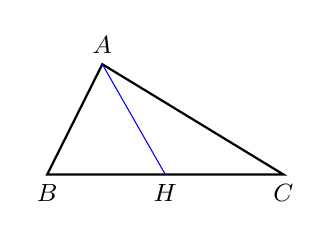
\begin{tikzpicture}[scale=1,font=\small]
\usetikzlibrary{calc}

\begin{scope}

\coordinate (b) at (0,0);
\coordinate (a) at (0.7,1.4);
\coordinate (c) at (3,0);

\draw[thick] (b) node[below] {$B$} -- (c) node[below] {$C$} -- (a) node[above] {$A$} -- cycle;

\coordinate (h) at ($(b)!0.5!(c)$);

\draw[blue] (h) node[black,below] {$H$} -- (a); % mediana
\end{scope}

\end{tikzpicture}

\end{minipage}
\end{esercizio}

\begin{esercizio}[Prove invalsi 2003]
\label{ese:2.100}
Da un triangolo equilatero $MNO$ di lato 6~cm viene tagliato via un 
triangolo equilatero di vertice in $O$ e lato 2~cm. Il perimetro del 
quadrilatero rimanente è \ldots
\begin{multicols}{5}
\begin{enumeratea}
\item 12~cm;
\item 14~cm;
\item 16~cm;
\item 18~cm;
\item 20~cm.
\end{enumeratea}
\end{multicols}
\end{esercizio}


\subsection{Risposte}

\begingroup
\hypersetup{linkcolor=black}

\paragraph{\ref{ese:2.54}.}
a)~V,\quad b)~F,\quad c)~V,\quad d)~V,\quad e)~F.

\paragraph{\ref{ese:2.99}.}
b.

\paragraph{\ref{ese:2.100}.}
c.

\endgroup
